\chapter{Production Plan}
\setlength{\parindent}{15pt}
\label{ch:prod_plan}

In case the finalised concept will be produced in series, a production plan will prove to be useful to show the required activities to build the Hybrid UAV. The production plan shows which steps need to be taken successively when building the aircraft, and which steps can be done concurrently. This production plan is created for a series production of 500 units. Figure \ref{fig:pp_top} shows the top level production plan for The Winged Quadcopter.

\begin{figure}[H]
    \centering
    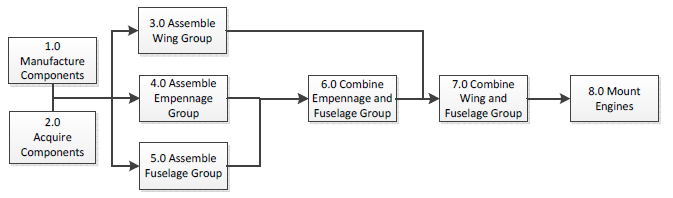
\includegraphics[width=\textwidth]{Production/Figures/Summary}
    \caption{Top Level Production Flow Diagram}
    \label{fig:pp_top}
\end{figure}

Looking at the top level, all of the required parts are acquired or manufactured first. Next, the three main groups of the aircraft can be constructed simultaneously, namely the fuselage, empennage and wing. Once these are constructed the assembly can begin, starting with the attachment of the empennage to the fuselage. This is followed by the attachment of the wing to the fuselage. This order has been chosen because the wings will complicate the process by taking up a lot of space. The engines are mounted last in order to minimise the risk of damaging them or the UAV during production.

The part manufacture is seen in \autoref{fig:pp_manu}. There are three different materials that need to be manufactured. The first branch is the branch for the manufacturing of glass fibre parts. These parts will be used for the construction of the fuselage. The three separate parts will all need to be laminated, using moulds that need to be made beforehand. Once the glass fibre has been laminated, rough edges need to be sanded off for a better finish. To make sure the parts are good enough, a final flaw detection needs to be done to find imperfections. The second branch is for the manufacturing of foam parts for the wing. The foam will be bought in blocks, and these blocks will be cut into sections corresponding to the distances between ribs. When the blocks are the correct length, the inner side of the wing skin will be cut. Finally, the outer side will be wire cut as well, showing a skin in the shape of a wing. The last branch is for the manufacturing of the carbon parts. The only carbon parts needed to be manufactured are the ribs. To make the ribs, they will be cut out of plates of carbon. After the cutting, these ribs also have to be sanded to have a smooth finish.

\begin{figure}[ht]
    \centering
    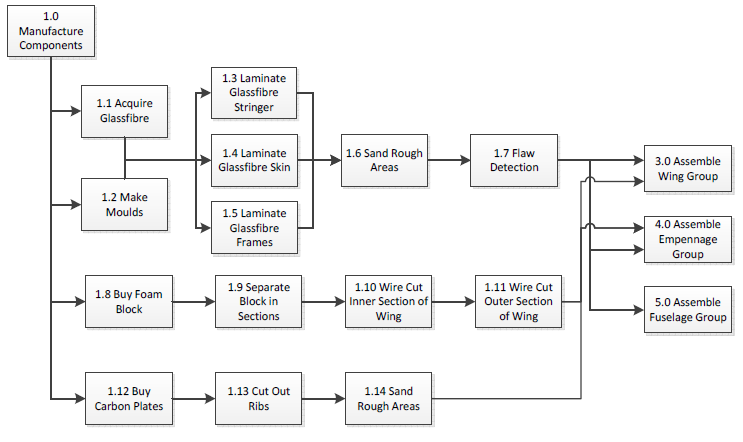
\includegraphics[width=\textwidth]{Production/Figures/10}
    \caption{Top Level Production Flow Diagram}
    \label{fig:pp_manu}
\end{figure}

The wing assembly is shown in \autoref{fig:pp_2}. Here, the wing structure is constructed by creating a spar and rib base for all other components to be fixed to. This includes attaching the foam skin to the structure, preserving the possibility to access the inside to mount components. The detailed base construction process is seen in \autoref{fig:pp_23}. It should be noted that this exact process is repeated for the construction of the vertical and horizontal tail bases. Next, parts such as control surfaces or engine mounts are constructed and mounted onto the base. Finally, an outer paint layer is added to the foam skin to ensure a smooth surface and protection against the environment.

\begin{figure}[H]
    \centering
    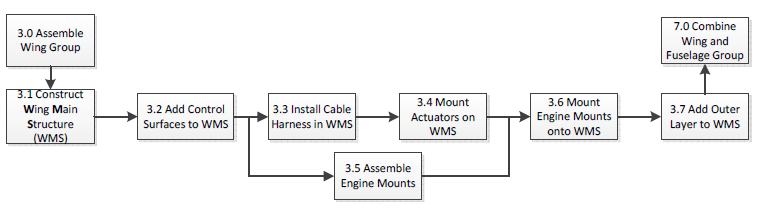
\includegraphics[width=\textwidth]{Production/Figures/30}
    \caption{Wing Assembly Flow Diagram}
    \label{fig:pp_2}
\end{figure}

\begin{figure}[H]
    \centering
    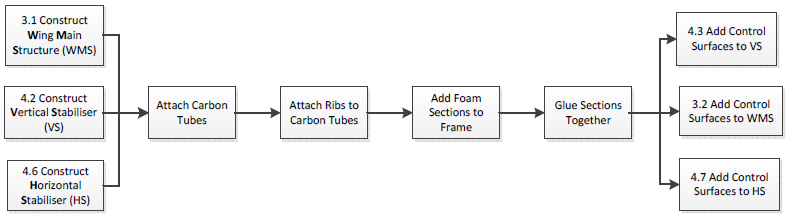
\includegraphics[width=\textwidth]{Production/Figures/3040}
    \caption{Main Structure Assembly Process}
    \label{fig:pp_23}
\end{figure}

The detailed empennage assembly is shown in \autoref{fig:pp_3}. This production stage comprises three parallel processes, namely the construction of the vertical and horizontal stabilisers, as well as of the empennage base. These are then assembled together, after which the actuators are mounted onto the base and connected to the control surfaces. The stage ends with the addition of an outer paint layer to the entire empennage.

\begin{figure}[H]
    \centering
    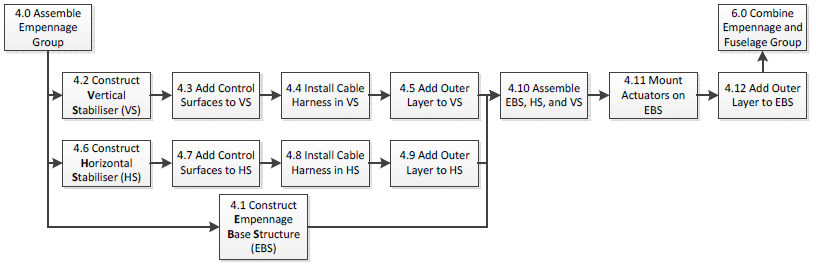
\includegraphics[width=\textwidth]{Production/Figures/40}
    \caption{Empennage Assembly Flow Diagram}
    \label{fig:pp_3}
\end{figure}

The fuselage structural assembly is described in a general manner in \autoref{fig:pp_4}. A detailed description of the installation of the electronics in the fuselage is shown in \autoref{fig:pp_5}. The structural assembly consists of constructing the fuselage base and payload bay in parallel, and then assembling them together. The rubber landing gear is mounted afterwards making it easier to assemble the payload bay beforehand. With the undercarriage installed, from this stage on the UAV will not require any additional structural supports during production. Finally the skin is attached to the fuselage structure. 

\begin{figure}[H]
    \centering
    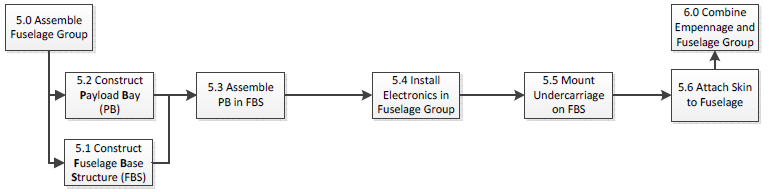
\includegraphics[width=0.9\textwidth]{Production/Figures/50}
    \caption{Fuselage Structure Assembly Flow Diagram}
    \label{fig:pp_4}
\end{figure}

The installation of the electronics consists of installing the cabling and the control computer first. The control computer will make it possible to test all the electrical components on the UAV, such as the actuators or motors. Performing these tests immediately after the installation of each electrical component will make it easier to fix or replace them if needed. Next the sensors and communication system are mounted on the fuselage.

\begin{figure}[H]
    \centering
    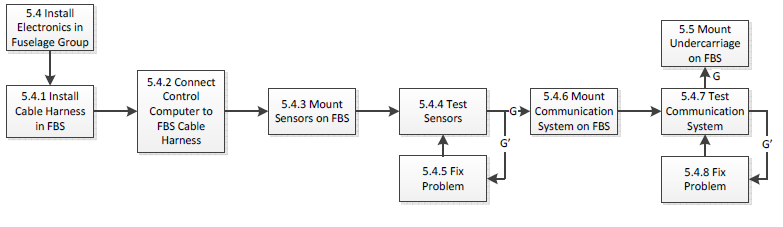
\includegraphics[width=\textwidth]{Production/Figures/54}
    \caption{Fuselage Electronics Assembly Flow Diagram}
    \label{fig:pp_5}
\end{figure}

Next, the empennage is assembled with the fuselage first (\autoref{fig:pp_6}), followed by the assembly of the fuselage with the wings(\autoref{fig:pp_7}). Both these processes consist of joining the structures, connecting the cable harnesses, and testing all the connections and actuators.

\begin{figure}[H]
    \centering
    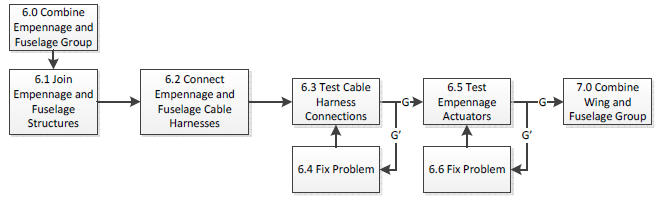
\includegraphics[width=0.9\textwidth]{Production/Figures/60}
    \caption{Fuselage and Empennage Joining Flow Diagram}
    \label{fig:pp_6}
\end{figure}

\begin{figure}[H]
    \centering
    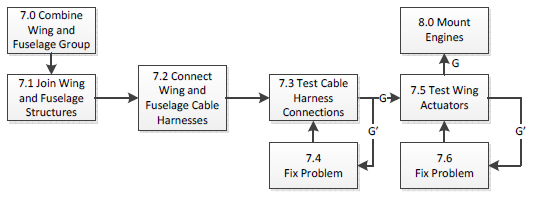
\includegraphics[width=0.8\textwidth]{Production/Figures/70}
    \caption{Fuselage and Wing Joining Flow Diagram}
    \label{fig:pp_7}
\end{figure}

The last step (\autoref{fig:pp_8}) involves mounting the engines to the engine mounts on the wings. The engines are heavy, hence attaching them last will make it easier to handle the product during the preceding production stages. In addition, there will be a lesser risk of damaging the UAV or the engines themselves in case of improper handling.

\begin{figure}[H]
    \centering
    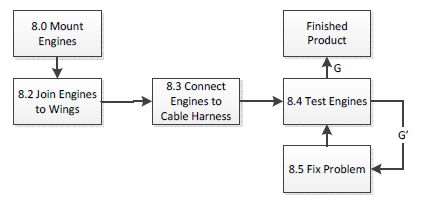
\includegraphics[width=0.6\textwidth]{Production/Figures/80}
    \caption{Engine Mounting Flow Diagram}
    \label{fig:pp_8}
\end{figure}

\nomenclature[A]{WMS}{Wing Main Structure}
\nomenclature[A]{VS}{Vertical Stabiliser}
\nomenclature[A]{HS}{Horizontal Stabiliser}
\nomenclature[A]{EBS}{Empennage Base Structure}
\nomenclature[A]{PB}{Payload Bay}
\nomenclature[A]{FBS}{Fuselage Base Structure}





